\section{Wave Equation in 1+1 Dimensions with Periodic Boundary Conditions}
\label{sec:simple_wave}

In order to accomplish our objective, first we need to develop code that can solve hyperbolic PDE's in 1+1 dimensions. To accomplish that goal, we will start by solving the wave equation in 1+1 dimensions with Cauchy initial conditions and periodic boundaries ($\Phi(t,x) = \Phi(t,x+L)$, where $L$ is the length of our system).

We will be solving this equation in its PDE system form (equation \eqref{eq:simple_wave_system}) with 2nd-order accuracy in space and 1st-order accuracy in time, using the initial conditions

\begin{align}
    \begin{array}{@{}l@{}}
        \Phi(0,x) = \sin(2\pi x),
        \\
        \Pi(0,x) = 2\pi \cos(2\pi x),
    \end{array}
    \label{eq:sin_IC}
\end{align}

\noindent
and periodic boundary conditions of length $L = 1$. 

In order to be able to do convergence tests, we will solve this equation with a resolution of 50, 100, 200, 400, and 800 points, which we compare two by two to give us an error estimation. These combinations will be directly used in the pointwise convergence under the names "low resolution", "medium resolution", "high resolution" and "higher resolution". We can then compare these error estimates two by two, calculating the norm convergence. These will go under the name "low resolution", "medium resolution" and "High resolution".

The norm convergence of the results is represented in figure \ref{fig:norm_simple_wave_2nd_order} and the pointwise convergence as a function of time for the point $x=0$ is represented in figure \ref{fig:point_simple_wave_2nd_order}.

\begin{figure}[t!]
    \centering
    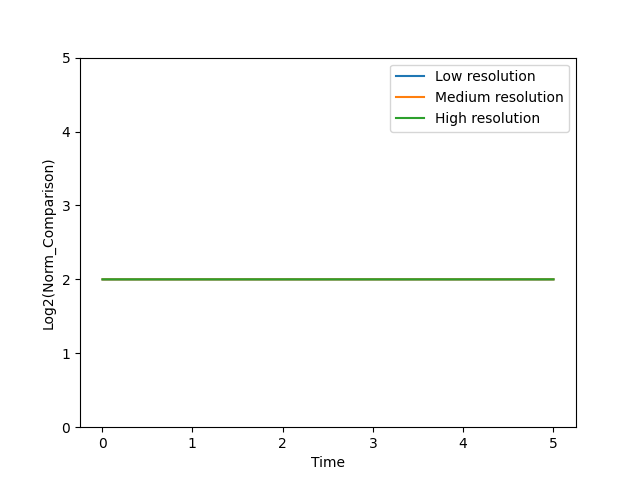
\includegraphics[width=\columnwidth]{Images/simple_wave-2nd-norm.png}
    \caption{Norm convergence of the solution to the wave equation in 1+1 dimensions with periodic boundary conditions and initial conditions represented in equation \eqref{eq:sin_IC} in the 2nd order accurate in space and 1st order accurate in time code}
    \label{fig:norm_simple_wave_2nd_order}
\end{figure}

\begin{figure}[t!]
    \centering
    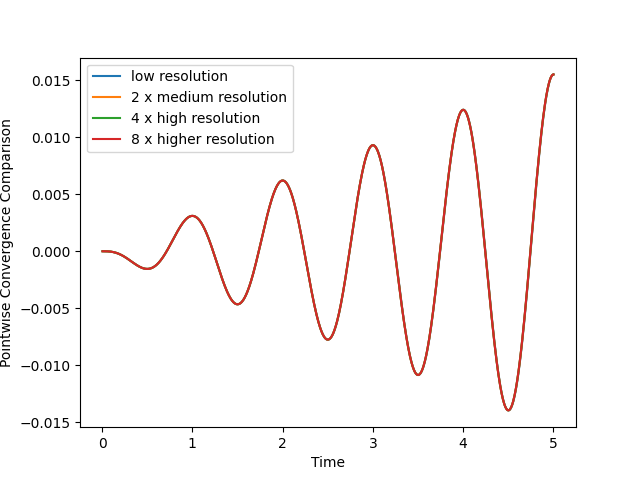
\includegraphics[width=\columnwidth]{Images/simple_wave-2nd-point.png}
    \caption{Pointwise convergence for $x = 0$ of the solution to the wave equation in 1+1 dimensions with periodic boundary conditions and initial conditions represented in equation \eqref{eq:sin_IC} in the 2nd order accurate in space and 1st order accurate in time code}
    \label{fig:point_simple_wave_2nd_order}
\end{figure}

The intensity plot of the solution is shown in figure \ref{fig:intensity_simple_wave_2nd_order}.

\begin{figure}[t!]
    \centering
    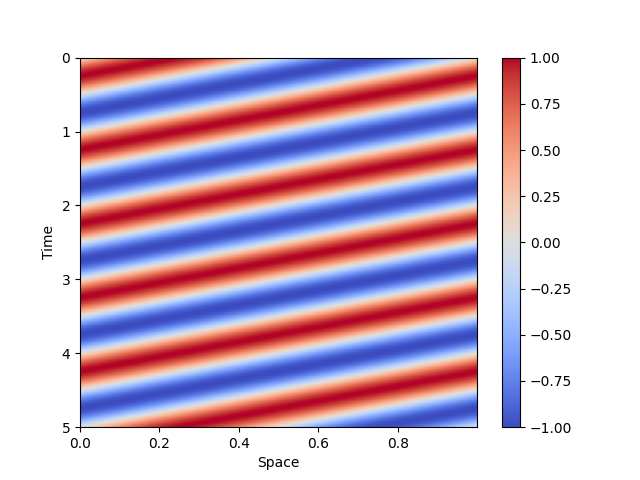
\includegraphics[width=\columnwidth]{Images/simple_wave-2nd_order-Intensity.png}
    \caption{Intensity plot of the solution to the wave equation in 1+1 dimensions with periodic boundary conditions and initial conditions represented in equation \eqref{eq:sin_IC} in the 2nd order accurate in space and 1st order accurate in time code}
    \label{fig:intensity_simple_wave_2nd_order}
\end{figure}

As we can observe in figures \ref{fig:norm_simple_wave_2nd_order} and \ref{fig:point_simple_wave_2nd_order}, the code shows a clean convergence for this solution in both convergence tests. 

Doing exactly the same procedure with 4th-order accuracy in space and 1st-order accuracy in time, we get similar results that are presented in the appendix. These results have a smaller error than the 2nd-order ones by two whole orders of magnitude, as they should have.

Since our results are very promising, we are ready to tackle harder problems.